
%%% Local Variables:
%%% mode: latex
%%% TeX-master: "../../doktorarbeit"
%%% End:
\chapter{The effects of rotation}
In this chapter we study the effects rotation have on the GW signal. 
We present three models based on the same progenitor, two rotating models and one non-rotating.
This allows us to study how the signal GW is effected by rotation. 


\section{Supernova Models}
We present the GW signal from three models based on the progenitor of
\cite{heger_05}, which is a solar-metallicity star with a ZAMS mass of $15 \msun$.
The progenitor was developed, taking into account the effects of magnetic fields and rotation,
from ZAMS to the onset of iron-core collapse. The inclusion of magnetic fields lead to an overall
reduction of the final rotation rate of the iron core, compared to a star evolved without magnetic
fields. The main difference between the three models is their rotation profiles. One of the models
uses the profile of the progenitor (m15r), an other has a enhanced rotation profile (m15fr),
in the last model the rotation rate has been set to zero throughout the star (m15nr)
In \fig{figp2:rot} we show the rotation profiles of m15fr and m15fr.
\begin{itemize}
\item \textbf{m15fr:} The rotation profile of model m15fr has, by hand, been set to a constant rotation rate of 0.5 rad/s
throughout the inner core of the star. At a radius of 1731 km the rotation profile changes
to a linearly decaying profile (\fig{figp2:rot}). The model was simulated using the Yin-Yang grid, the 
two grid patches had an initial resolution of 400 cells, 56 cells and 144 cells in the radial, polar and
azimuthal directions, respectively. This corresponds to a 2 degree angular resolution. 
After the initial shock expansion halts around $60$ ms post bounce the average shock radius decreases slightly.
Between $\sim 80 - 160$ ms post bounce the shock front is on average more or less stationary. 
The shock starts to expand roughly $160$ ms after core bounce and soon after shock revival sets in.
The average shock reaches $2000$ km around $\sim 330$ ms after core bounce.
In the time before shock revival, the post-shock flow is dominated by a strong spiral SASI mode. The SASI sets in around
$\sim 100$ ms post bounce.
\item \textbf{m15r:} The initial rotation profile of model m15r is exactly that of the progenitor \citep{heger_05}, without
any artificial changes made by hand. The rotation profile as a function of radius can be seen in \fig{figp2:rot}.  
The model was simulated using the Yin-Yang grid, the two grid patches had an initial resolution of 400 cells, 
56 cells and 144 cells in the radial, polar and azimuthal directions, respectively. This corresponds to a 2 degree angular resolution.
For the first $\sim 80$ ms after bounce, the evolution of the average shock radius of model m15r closely resembles the
one seen in model m15fr. However, around $100$ ms the average shock radius starts to decrease. Unlike model m15fr, strong 
SASI activity does not develop in model m15r, the flow in the post-shock region is instead dominated by hot-bubble convection. There
is, however, some low amplitude dipole deformation of the shock front (see \fig{figgp2:sasi}).
The average shock radius continue until
$\sim 200$ ms post bounce when the Si-O shell interface falls through the shock. The decrease density in front of the shock leads
to decreased ram pressure and a transient period of shock expansion. At $\sim 240$ ms post bounce the expansion subsides and
the shock front once more begins to retreat, a trend which continues until the end of the simulation.  
\item \textbf{m15nr:} In model m15nr the initial rotation rate was set to zero at all radii. The model was simulated using the Yin-Yang grid, the
two grid patches had an initial resolution of 400 cells, 28 cells and 72 cells in the radial, polar and
azimuthal directions, respectively. Which means that model m15nr was simulated with an angular resolution that is
two times coarser than the other two models (4 degrees). Initially the shock expands and reaches a local maximum around $60$ ms after bounce,
from this point the shock radius steadily decreases until the Si-O shell interface falls through the shock. The decreased accretion rate
leads to a transient period of shock expansion, until the shock eventually starts to recede once more. Except for the fact that
the average shock radius is generally larger in model m15nr, model m15nr is similar to model m15r in terms of the evolution of the average shock
radius. However, unlike model m15r, model m15nr develops strong SASI activity. In this model the SASI activity is dominated by the sloshing mode.
The mode develops around $\sim 120$ ms after core bounce and peaks around $\sim 230$ ms post bounce. After the peak in activity 
the SASI mode gradually decays towards the end of the simulation.   
\end{itemize}
\begin{figure}[H!]           
\centering                            
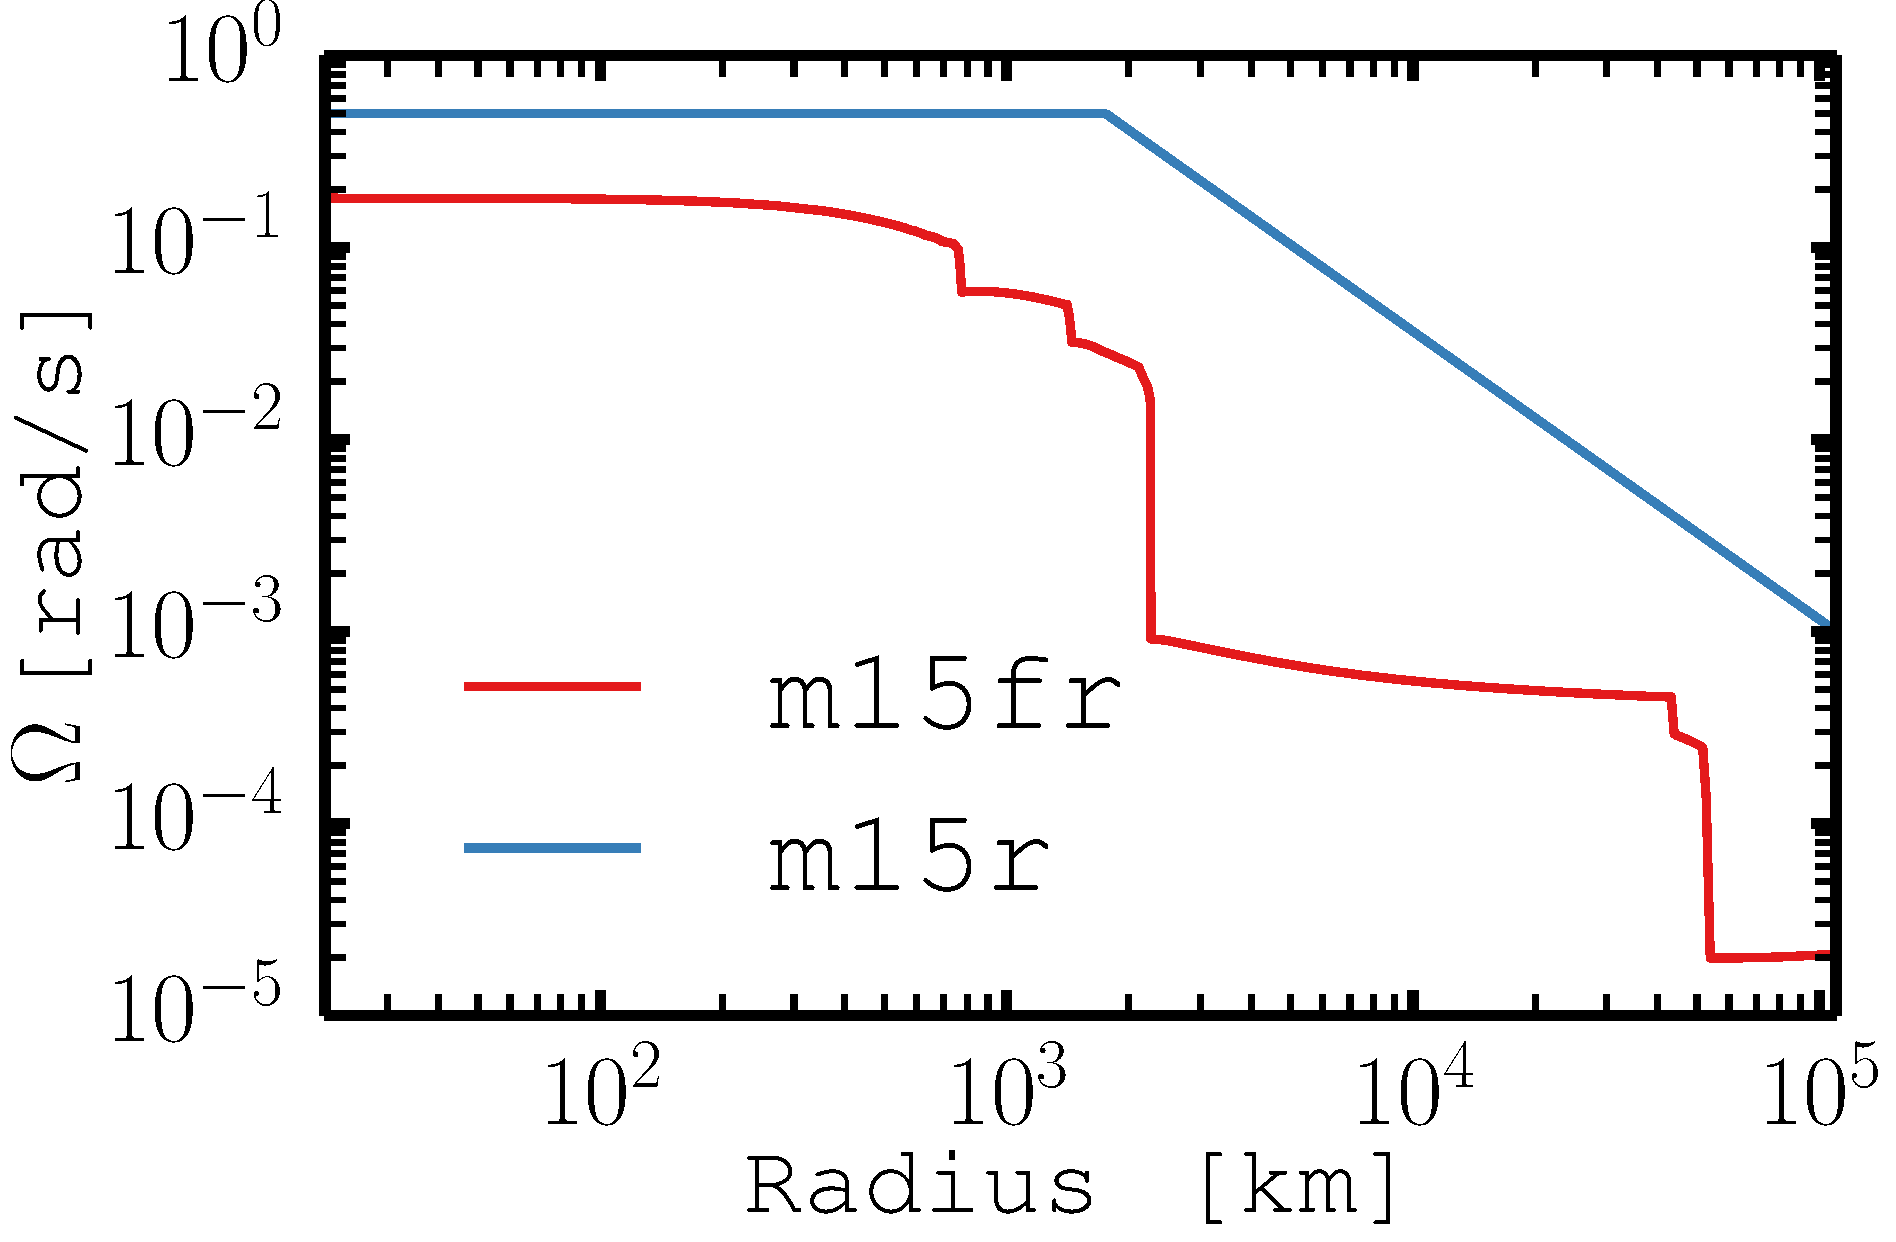
\includegraphics[width=0.99\textwidth]{./images/paper2/rot.pdf}
\caption{The radial rotation profiles for the two rotating models. The red line represents model 
m15fr and the blue line represents m15r. \label{figp2:rot}}
\end{figure}
\begin{figure}[H!]         
\centering                            
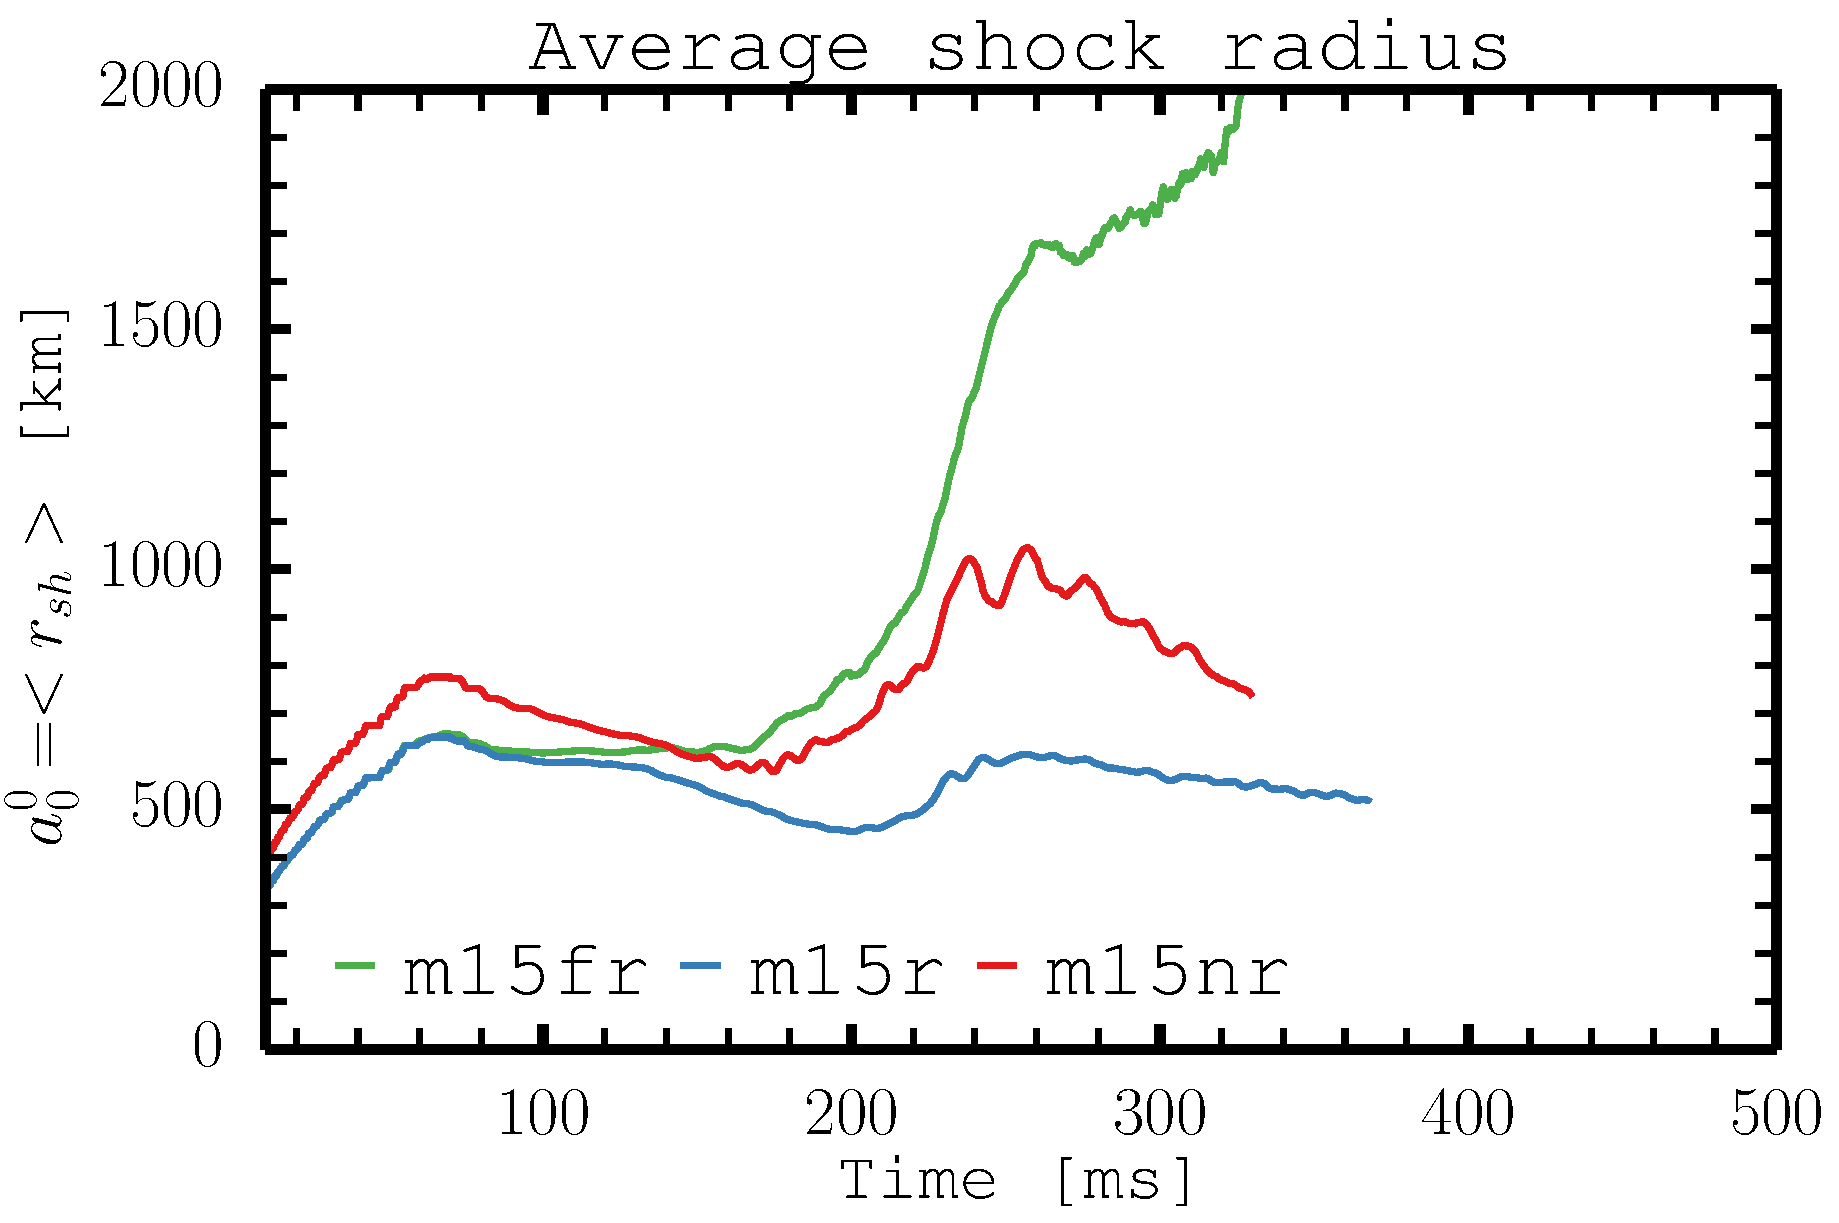
\includegraphics[width=0.99\textwidth]{./images/paper2/rsh.pdf}
\caption{Average shock radius for model m15fr (green), m15r (blue), and m15nr (red) as a function of 
time after core bounce. The average shock radius is defined as the $(l,m) = (0,0)$ expansion coefficient of the shock surface into 
spherical harmonics (\eq{eq:alsph}). \label{figp2:rsh}}
\end{figure}
\begin{figure}[H!]         
\centering                            
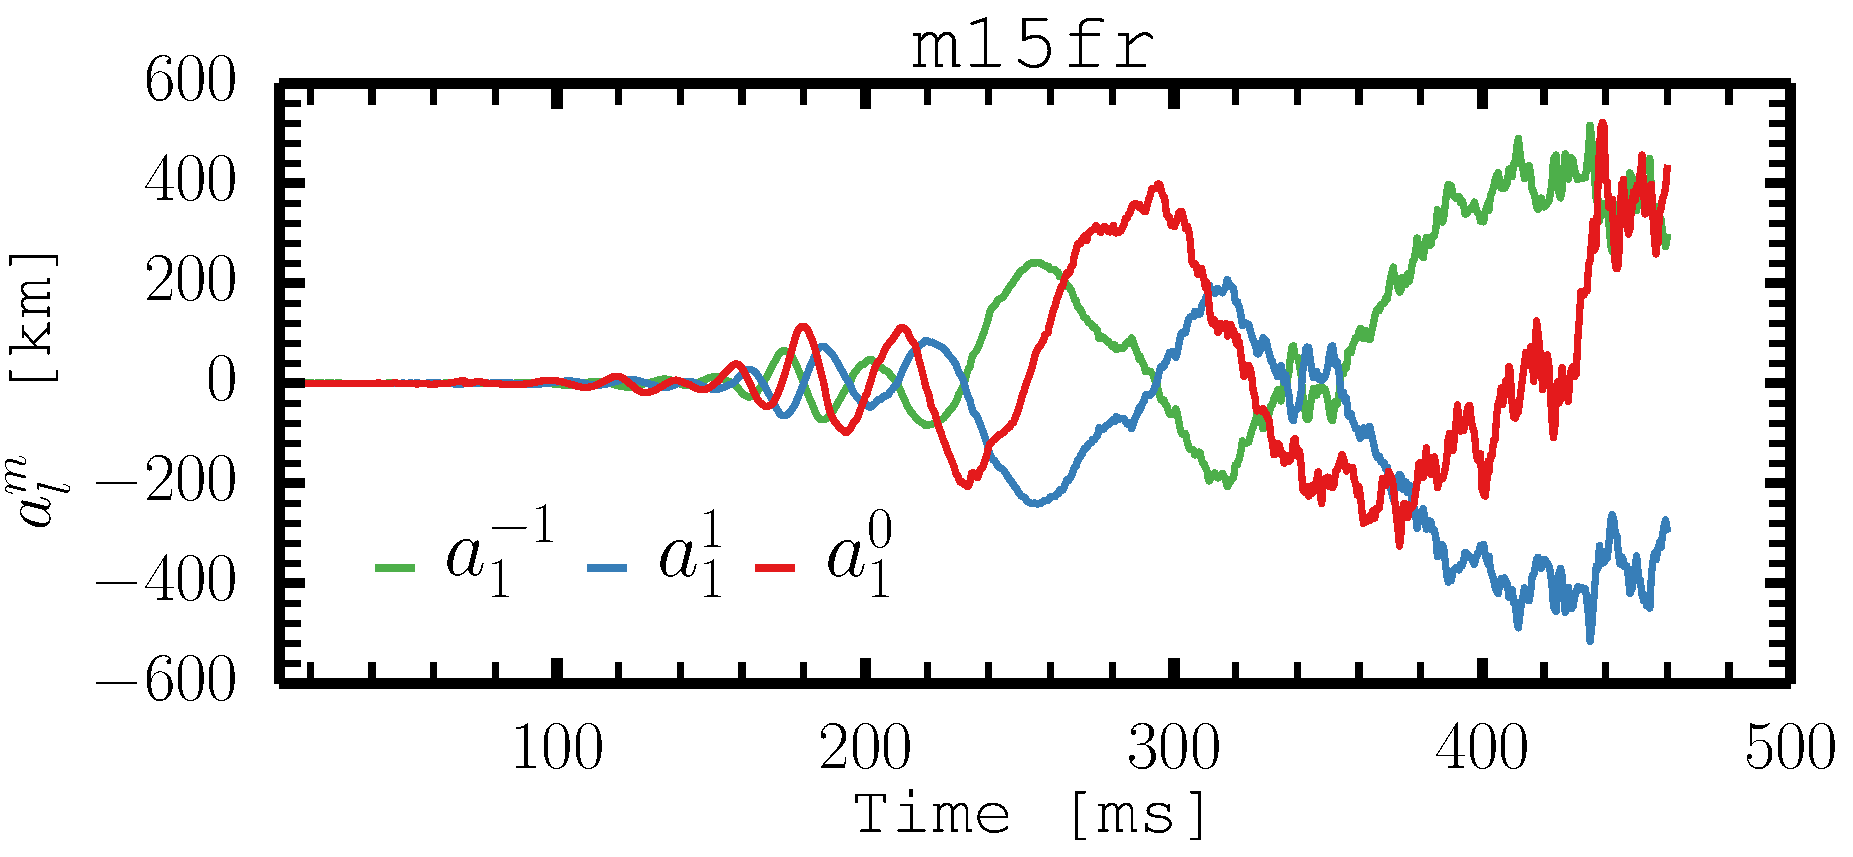
\includegraphics[width=0.9\textwidth]{./images/paper2/sasi_fr.pdf}
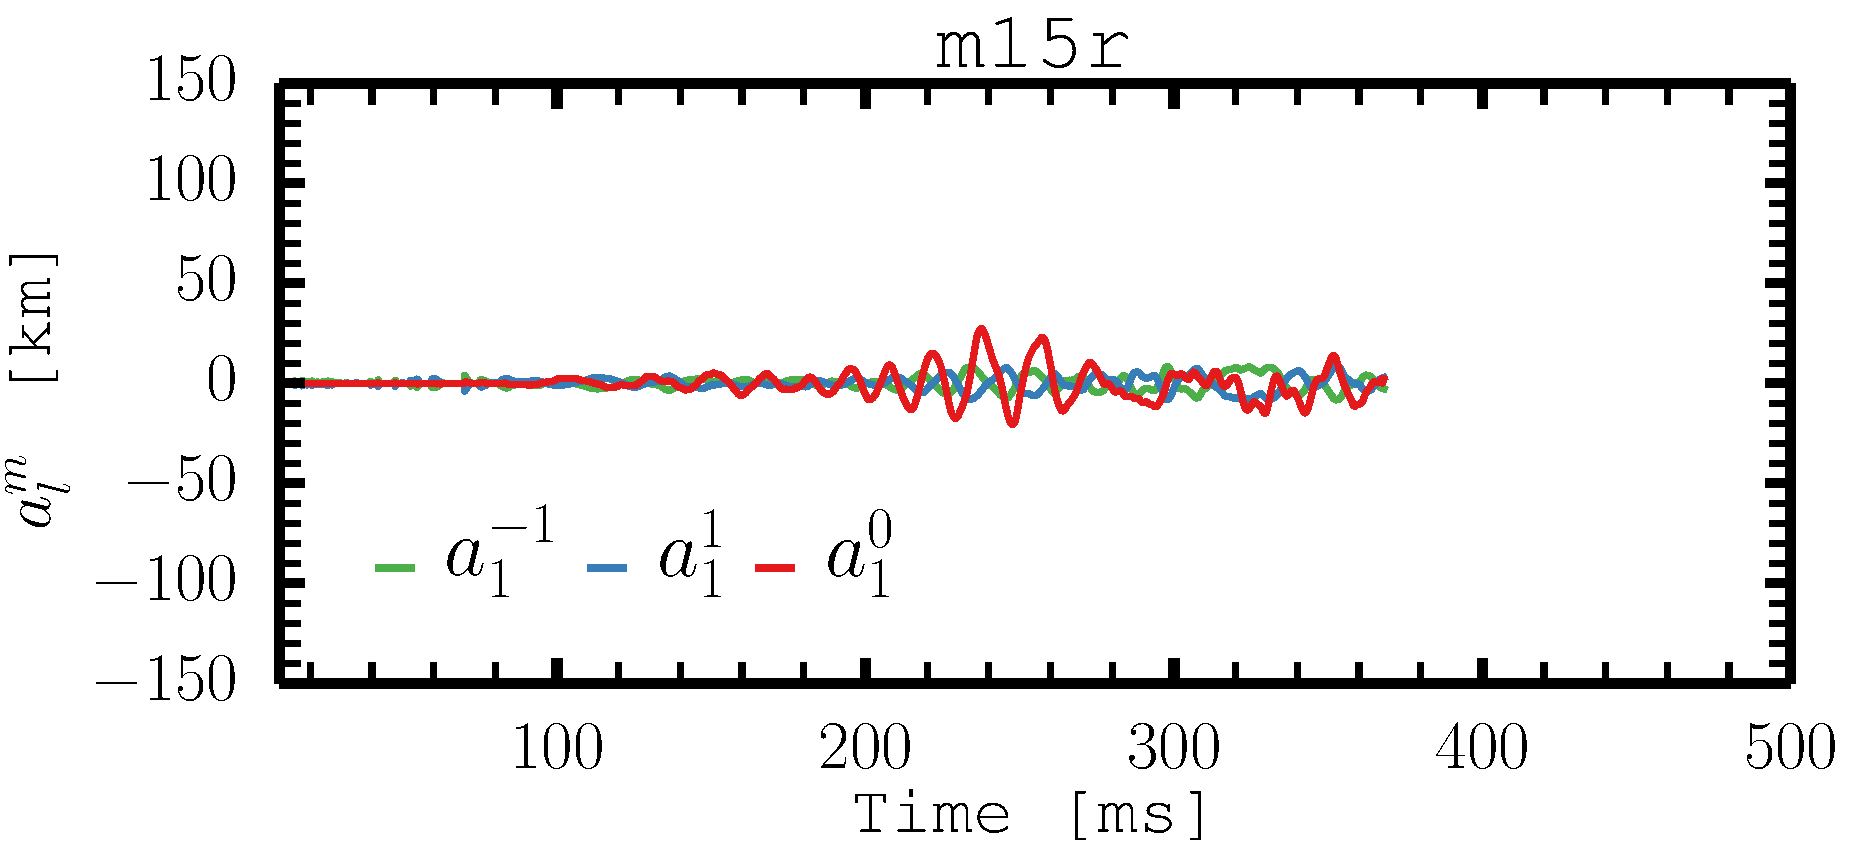
\includegraphics[width=0.9\textwidth]{./images/paper2/sasi_r.pdf}
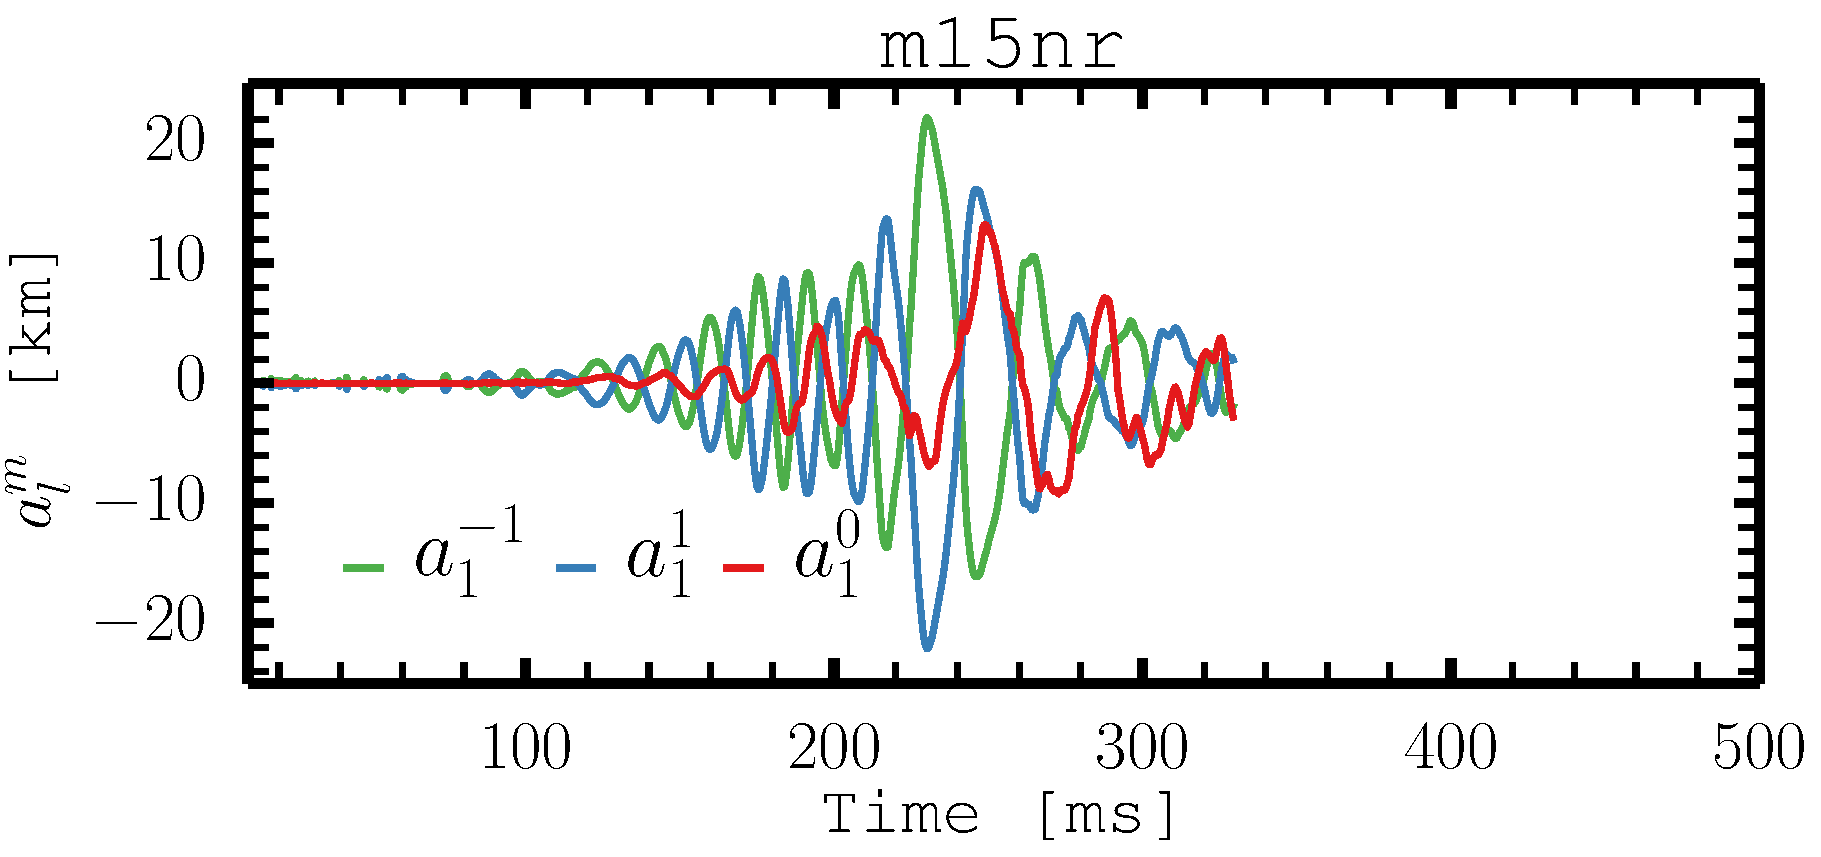
\includegraphics[width=0.9\textwidth]{./images/paper2/sasi_nr.pdf}
\caption{The $(l,m) = (1,0)$, $(1,1)$, and $(1,-1)$ coefficients of the decomposition of the shock surface into spherical harmonics
as a function of time after bounce, see \eq{eq:alsph}. From the top to bottom: Model m15fr, model m15r, and model m15nr. \label{figp2:sasi}}
\end{figure}

\section{Results}
\subsection{Qualitative description of the gravitational wave signals}
The GW signals from the rotating models do not qualitatively differ significantly from
the signals presented in chapter~\ref{ch:firstpaper}. In \fig{figp2:amps} we show the
GW amplitudes generated by asymmetric mass motions for models m15fr, m15r and m15nr.
The two columns shows the amplitudes for two different observer orientations,
the right and left Colon represent observers situated along the x-axis (equator) and z-axis (pole) of the Yin grid-patch,
respectively. The rows are order by progenitor, in order of decreasing initial rotation, and from the top
shows m15fr, m1fr and m15nr. Vertical lines indicates episodes of strong SASI activity.
The corresponding amplitude spectrograms (see \eq{eqSA:STFT}) for a sliding window of $50 \, \mathrm{ms}$ are shown 
in Fig.~\ref{fig:totspec}. The spectrograms show the sum of the squared Fourier
components of the cross and plus polarisation modes,
$STFT[{A_+}]^2 + STFT[{A_{\times}}]^2$. Before applying the
DFT we convolve the signal with a Kaiser window with shape parameter $\beta = 2.5$. Frequencies
below $50 \, \mathrm{Hz}$ and above $1100  \, \mathrm{Hz}$ are filtered out of the resulting spectrograms. 

In all three models, an initial phase of quiescence is followed by a phase of rather stochastic emission, 
during with the typical amplitudes are on the order of a few cm. Model m15fr have the largest amplitude, of the three
models, but at the same time the non-rotating model (m15nr) show larger amplitudes than the moderately rotating model (m15r).
There seems to be no clear correlation between the strength initial rotation rate and the strength of the GW emission. 
The spectrograms (\fig{figp2:spec)} show the familiar low-frequency and a high-frequency components that we saw in the
four models presented in chapter~\ref{ch:firstpaper}.

During the SASI phase of m15fr, we see a low-frequency signal component in addition 
to the high-frequency stochastic component. Both strong low-frequency and high-frequency
emission is visible in the upper row of \fig{figp2:spec}. Both signal components
are broader in model m15fr than in the other two models, to the point where the two components almost
overlap. After the shock starts to expand the overall GW amplitudes are somewhat reduced, but
both low-frequency and high-frequency emission continues until the end of the simulation.

Of the three models, model m15r produces the weakest GW signal. The GW amplitudes
never exceeds $1.5$ cm, for both observer directions. Furthermore, between 180 and 250 ms post bounce there
is a period of reduced emission. High-frequency emission almost completely subsides during this period,
and the low frequency emission is rather weak. Around $\sim 250$ ms post bounce high-frequency emission 
sets in once more, and at the same time the low-frequency emission ceases. 

In the non-rotating model (m15nr) the GW signal is slower to develop, compared to the two rotating models.
Around $\sim 125$ ms after core bounce weak low-frequency emission sets in. By $\sim 150$ ms after bounce
high-frequency emission develops. Except for two minimums at $\sim 240$ and $\sim 275$ ms post bounce, the
signal in general terms remains unchanged until the end of the simulation, with both the high-frequency
and low-frequency component visible in the spectrograms for the duration of the simulation.

\begin{figure}           
\centering                            
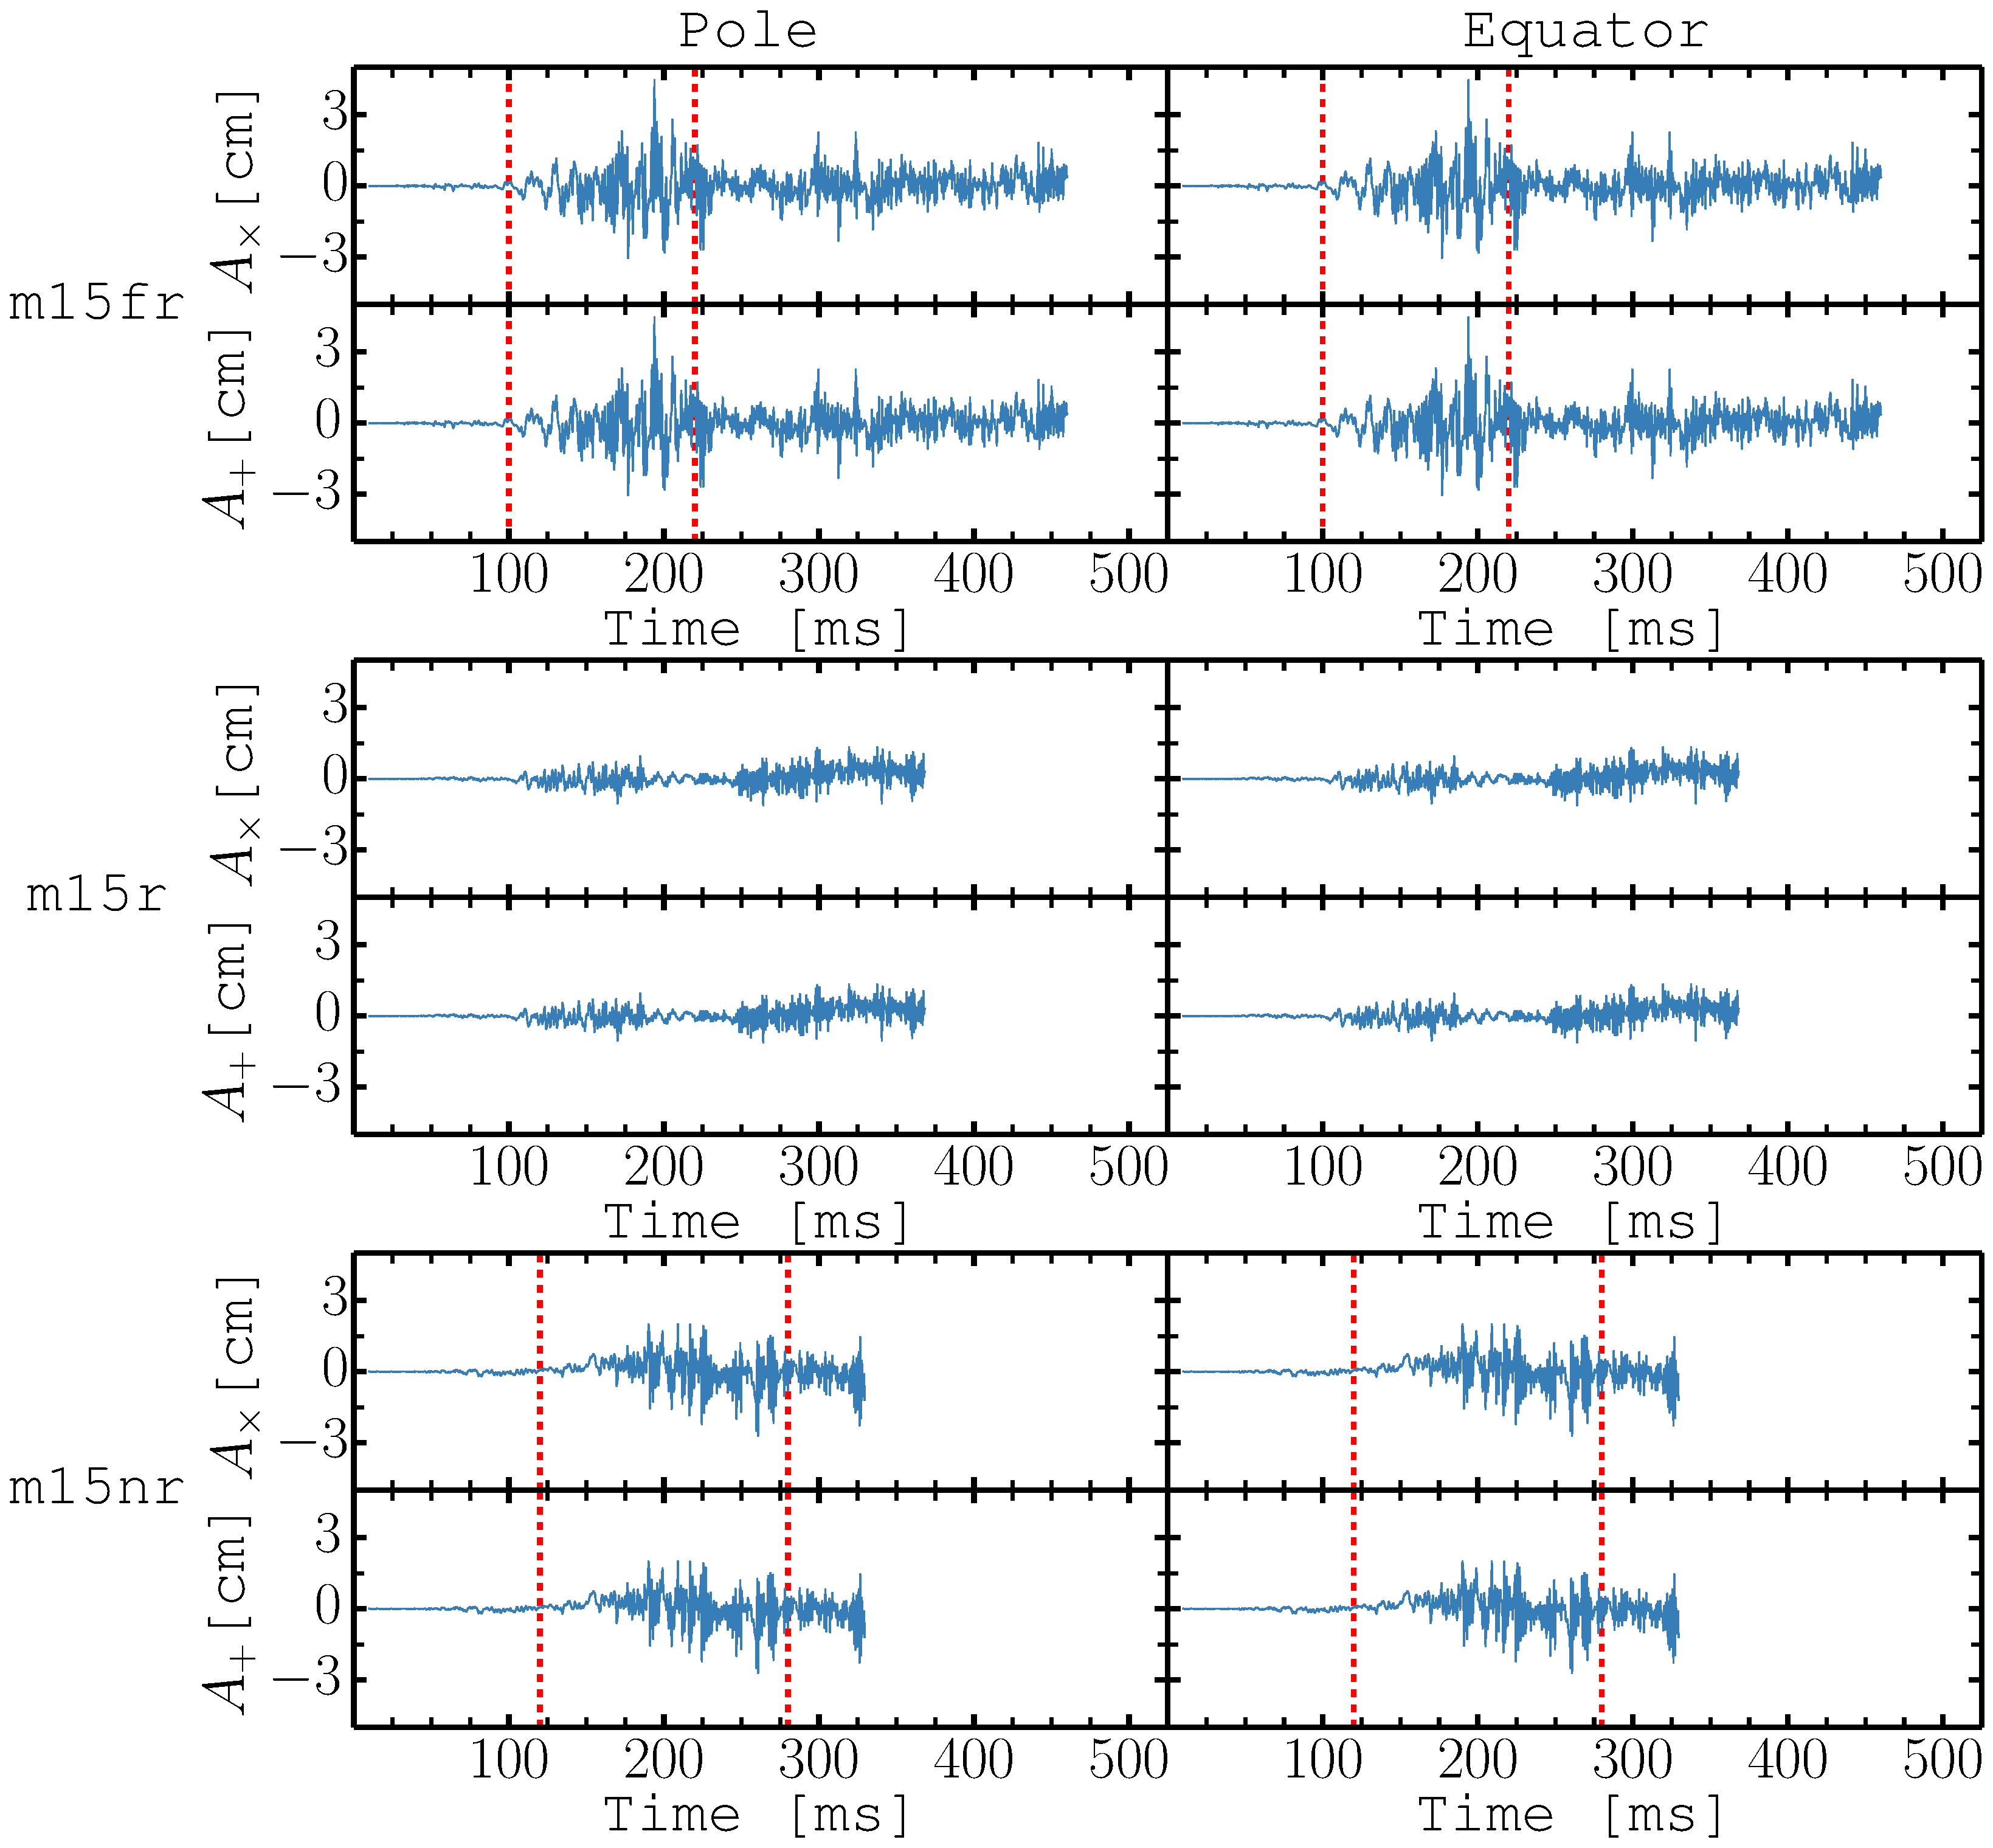
\includegraphics[width=0.99\textwidth]{./images/paper2/amps.pdf}
\caption{GW amplitudes $A_+$ and $A_\times$ as functions of time after core bounce.
  From the top: m15fr, m15r, and m15nr, respectively. 
  The two columns show the amplitudes for two different viewing angles: an observer
  situated along the $z$-axis (pole; left) and an other observer along the $x$-axis (equator; right) of the Yin grid patch, respectively.
  Episodes of strong SASI activity occur between the vertical red lines.  \label{figp2:amps}}
\end{figure}


\begin{figure}           
\centering                            
\includegraphics[width=0.99\textwidth]{./images/paper2/rotspec.pdf}
\caption{Amplitude spectrograms for a sliding window of 50 ms and two different observer
  directions, summed over the two polarisation modes 
  ($|\widetilde{A}_+|^2 + |\widetilde{A}_\times|^2$). The
  different rows show the results for models m15fr, m1fr, and m15nr. (top to bottom).
  The two columns shows the spectrograms for two different viewing angles, the right and left column represent
  observers situated along the z-axis (pole) and x-axis (equator) of the Yin grid, respectively.
  The time is given in ms after core bounce. Vertical lines bracket SASI episodes. All panels have been normalised by the same global factor.
  The colour bar is given in a logarithmic scale. \label{figp2:spec}}
\end{figure}


During this phase the shock front first contracts and
then expands again. During the same time period the  deformation, with $m=0$, 
of the shock increases in strength, reaches its maximum and subsequently decays again, see \fig{figp2:sasi}.
